\chapter{Approach}
\label{ch:approach}
%%%%%%%%%%%%%%%%%%%%%%%
% - description of the designed system
% - analysis and review of the current software architecture
% - gerne in die Tiefe gehen
%%%%%%%%%%%%%%%%%%%%%%%

In this chapter we give an overview to the design of the Basilisk platform.
We will explain the different processes used in the platform in section \ref{sec:main_services}.
In section \ref{sec:architecture_review} we will analyze and review the current software architecture and implementation status of the Basilisk platform.
\\

\todo[inline]{mehr roter Faden, Verbindung zw den genannten Punkten}
The purpose of the Basilisk platform is to provide an easy way to continuously perform benchmarks on \tsp{}.
Triplestores are often developed in teams who collaborate in Git repositories.
Releases of those \tsp{} are then published on \gh{} or as a Docker image on \dockh{}.
The idea is that the Basilisk platform will automatically check for a new release of a registered \ts{} repository and will then perform benchmarks on this release.

Benchmarks are also relevant during the development process.
A benchmark performed automatically, for example, when a new pull request is added, is a good way to estimate if a newly developed feature will impact the performance of the \ts{} before the changes are merged.

On the Basilisk platform, a user can register a \ts{} for a continuous benchmark by setting up a hook to the repository on \gh{} or \dockh{}.
The repository will then be observed by the Basilisk platform.
If there is a new release of the \ts{}, Basilisk will generate a new benchmark job.
This benchmark job will then be executed by fetching and building a new Docker container, containing the newest release of the \ts{}.
On this container the benchmark will be performed.
The measured results of the benchmark will be stored in a \ts{} and are then available through the web frontend for review.
\\

The basic architecture pattern of the Basilisk platform is the microservice architecture (see chapter \ref{sec:microservice_architecture} for a short description). 
This means that the platform is divided into multiple services on which the workload and the different tasks are divided.
The services can be run on different hardware systems and they interact with each other via the RabbitMQ (\ref{sec:rabbitmq}) message queue system.
\\

\section{Programming Language and Frameworks}
\label{sec:prog_lang_and_framework}
All services of the Basilisk platform are implemented with Java and are using the Spring Boot framework.
The services use Java version 17 and Spring Boot version 2.6.6.

The package structure used for implementing the services is similar in all three services.
It is strongly influenced by the structure recommended for the Spring Boot framework.


%%%%%% MAIN SERVICES
\section{Main Services}
\label{sec:main_services}
The next sections explain the three main services, namely \acl{hcs} (section \ref{sec:hooks_checking_service}), \acl{jms} (section \ref{sec:jobs_managing_service}), and \acl{tbs} (section \ref{sec:ts_benchmarking_service}).

This explanation follows the flow of actions that happen while configuring a continuous benchmark and the actions that happen when a benchmark is initiated.

The explanations are based on provided diagrams, code review and analysis, and information provided by former developers of the project.
\\

Figure \ref{fig:basilisk_high_level_design_approach} gives an overview of the three microservices of the Basilisk platform.
It shows the most important messages send between the services and the interactions with \gh{} and \dockh{}.
\begin{figure}[tbph]
	\centering
	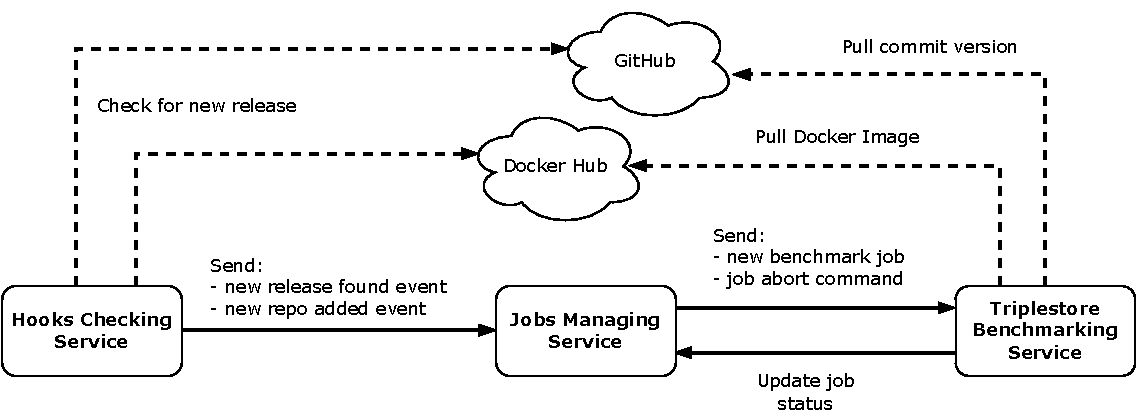
\includegraphics[width=1\textwidth]{figures/high-level-design-approach.pdf}
	\caption{Overview of the three microservices}
	\label{fig:basilisk_high_level_design_approach}
\end{figure}



\subsection{\acl{hcs}}
\label{sec:hooks_checking_service}
The main task of the \ac{hcs} is to observe \gh{} and \dockh{} repositories of \tsp{} for new releases or changes.

When a user wants to set up a new continuous benchmark, the \ac{hcs} needs to be informed which repository (\gh{} or \dockh{}) has to be observed for changes.
This happens through REST API calls to the \ac{hcs} providing the repository name and owner.
The \ac{hcs} will then create a hook for the repository to get notice about changes.
A hook is in general a piece of code or software that attaches itself to a software component to intercept messages and react to those messages, \eg, with function calls.
In the case of the \ac{hcs} the hooks can be seen as bookmarks for the repositories.
Each hook stores the latest known version of an repository.
The service will query the saved repositories regularly and compare their current version to the version stored in the hook.

When the \ac{hcs} notices a new release for a repository, it updates the corresponding hook to the newest version.
Then it sends a message about the new version to the \aclp{jrq} from which the \acl{jms} retrieves the message.

\subsubsection{API and Messaging}
\label{sec:hooks_api}
The \ac{hcs} is controlled by the user over a REST API.

The continuous checking of the repositories can be started and stopped over a REST endpoint.
The other most important endpoints are for adding and deleting \gh{} and \dockh{} repositories.
Figure \ref{fig:rest_apis_approach_hcs} shows these endpoints.
\begin{figure}[tbph]
	\centering
	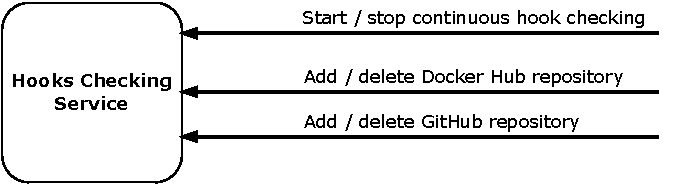
\includegraphics[width=.57\textwidth]{figures/rest-apis-approach-hcs.pdf}
	\caption{REST API of the \acl{hcs}}
	\label{fig:rest_apis_approach_hcs}
\end{figure}

The communication between the \ac{hcs} and the \acl{jms} is done over RabbitMQ (\ref{sec:rabbitmq}) messages, over the \aclp{jrq}.
The messages contain different events that can occur in the \ac{hcs}.
For example an event is send when adding or deleting a repository, or a new release is detected.


\subsection{\acl{jms}}
\label{sec:jobs_managing_service}
The main task for the \acf{jms} is to create benchmark jobs, when a new release was found by the \ac{hcs}.
Other important functionality of the \ac{jms} is the management of configurations needed for the benchmarks.
Lastly the \ac{jms} manages the status for running and pending jobs send to the \acl{tbs}.
\\

There are three configuration types needed.
First the platform needs the configuration for the \ts{}.
This configuration include for example the SPARQL endpoint as well as the user and password for the connection to the endpoint.
This is needed by the \iguana{} framework to properly connect to the \ts{} under test\cite{IguanaDocumentationConfiguration}.

Secondly the platform needs configurations for datasets and query configurations.
The dataset configuration simply consists of the dataset name and the URL for the location of the dataset.
The query configuration consists similarly of a name for the queries and the URL for the location of the query file.

These configurations are added over the REST API of the \ac{jms}.
\\

When the \ac{hcs} sends an event regarding a new release of a repository, the \ac{jms} will create benchmark jobs for the new release.
A benchmark job consists of the current version of the repository, a query configuration and a dataset.
For each event multiple benchmark jobs can be created.
For each query configuration and dataset one benchmark job will be created.

These benchmark jobs will then be send to the \acl{tbs} over the \acl{bjq}.

The management of the running and pending benchmark jobs is done over the REST API of the \ac{jms}.
When an endpoint is triggered, \eg, to abort a running job, the \ac{jms} sends an event to the \acl{tbs}.


\subsubsection{API and Messaging}
\label{sec:jobs_api}
The \ac{jms} communicates with the \ac{hcs} and the \acl{tbs} over RabbitMQ message queues.
The service receives repository events from the \ac{hcs} and sends benchmark job events to the \acl{tbs} over the \ac{bjq}.
\\

Interaction of the user is handled over the REST API.
The API offers endpoints for adding and deleting the different configurations of \tsp{}, datasets and queries
A second set of endpoints are for querying the job status of running and pending jobs, and for stopping individual jobs.
Figure \ref{fig:rest_apis_approach_jms} shows these endpoints.
\begin{figure}[tbph]
	\centering
	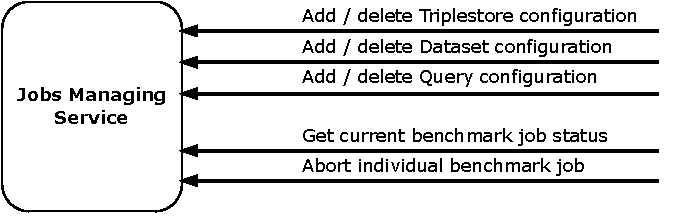
\includegraphics[width=.57\textwidth]{figures/rest-apis-approach-jms.pdf}
	\caption{REST API of the \acl{jms}}
	\label{fig:rest_apis_approach_jms}
\end{figure}


\subsection{\acl{tbs}}
\label{sec:ts_benchmarking_service}
The \ac{tbs} executes the benchmark jobs send by the \ac{jms} and saves the benchmark results to a \ts{}.

To execute a benchmark the service needs a running instance of the \ts{} under test on which the benchmark will be executed.
This instance is build from the information and configurations provided in the benchmark job.
The \ac{tbs} will query the provided repository (\gh{} or \dockh{}) for the version specified in the job.

If the repository is from \gh{}, the \ac{tbs} downloads the source code for the provided commit and searches for a Dockerfile.
It then builds and runs a Docker container from that Dockerfile.

If the repository is from \dockh{}, the \ac{tbs} pulls the image with the provided tag.
It then runs the image as a Docker Container.
\\

After starting the Docker Container the \ac{tbs} starts the \iguana{} framework.
\iguana{} will perform the benchmark with the provided configuration from the benchmark job.

When the benchmark is finished the results are written to a \ts{} called \acl*{jsts}

\subsubsection{API and Messaging}
\label{sec:benchmarking_api}
The \ac{tbs} has no REST API.
The service is controlled through the \ac{jms} by events send over RabbitMQ.

The events received from the \ac{jms} are new benchmark jobs and pause or abort commands for running benchmark jobs.
The \ac{tbs} sends short events containing the status of benchmark jobs, \eg, a job has started, or it has finished and the results are uploaded to the \acl{jsts}.



\section{Basilisk Frontend}
\label{sec:basilisk_frontend}
The Basilisk platform can be extended with a web frontend.
The frontend is implemented using JavaScript and the JavaScript framework Vue.js.

The idea is that the frontend functions as a graphical interface for the REST APIs of the three services explained in section \ref{sec:main_services}.
The user can set up new repositories, \tsp{} and datasets.
Further, the user can request information about current benchmark jobs, abort or remove pending jobs.
Lastly, the frontend can request and visualize the benchmarking results stored in the \acl{jsts}.



%%%%%% ARCHITECTURE REVIEW
\section{Architecture and Code Review}
\label{sec:architecture_review}
In this section, we review the architecture of the three services of the Basilisk platform.
We point out possible problems with the previous implementations and list missing implementations that need to be added.


\subsection{Code Refactoring}
\label{sec:code_refactor}
Code refactoring is the process of restructuring the source code of an application without changing its functionality \cite{fowlerRefactoringImprovingDesign2019a}.
During the code analysis some inconsistencies in the code style and duplicate code snippets have been found.
In other parts the code structure differed from the design patterns recommended for the Spring and Spring Boot framework.

In general, an in-depth code refactoring was recommended to increase readability and maintainability of the source code. 


\subsection{Management of Repositories and Configurations}
\label{sec:management_repo_config}
Previously, the observed repositories were managed and stored in the \ac{hcs} while the configurations for the \tsp{} were managed and stored in the \ac{jms}.
This made it difficult to internally link a repository to a \ts{} configuration, since they were stored in different services.

The previous implementations tried to solve this problem, by sending events about repository creations from the \ac{hcs} to the \ac{jms}.
This resulted in the duplication of the repository storage in both services.
This contradicted the idea of microservice, which should be separated as much as possible from each other.

Therefore we recommended restructuring the management of repositories.


\subsection{Creation and Management of Benchmarking Jobs}
\label{sec:creation_of_benchmark_jobs}
When a new release is found by the \ac{hcs}, the \acl{jms} will create and manage benchmarking jobs which will be executed by the \ac{tbs}.
Previously, the \ac{jms} had created multiple jobs.
For each query file a job was be created for each dataset.
This means that each dataset was mixed with each query file, which lead to queries executed on the wrong datasets.

A benchmark should only use a defined pair of a matching query file and dataset.
Therefore, the logic for creating the benchmark jobs had to be changed, as well as the data model for storing the benchmark jobs.


\subsection{Data Model Restructure}
\label{sec:review_data_model}
The \ac{jms} manages and stores the different configuration types needed for a benchmark job.

The configurations are stored in an internal database.
Figure \ref{fig:jms_db_schema} shows the previous database schema.

The schema had logical errors and was in parts incomplete.
In the following we list some inconsistencies and possible problems that we noticed:
\begin{itemize}
	\item The only way to identify a repository as \gh{} or \dockh{} repository was to check in the \ts{} configuration.
		If a repository was assigned to the false type, the resulting benchmark job was not executable, because \gh{} and \dockh{} need to be handled differently during a benchmark as explained in section \ref{sec:ts_benchmarking_service}.
	
	\item Each \ts{} configuration could have exactly one \gh{} or \dockh{} repository.
		This means that for every repository a new \ts{} configuration had to be added.
		There are less duplicate configurations if multiple repositories point to the same configuration.
		For example, a hook is set up to observe a \gh{} repository for new releases and another hook is set up to observe the same \gh{} repo for pull requests.
		In this case both hooks are using the same \ts{} configuration, since it is the same \ts{} which gets benchmarked.
		
	\item As explained in section \ref{sec:creation_of_benchmark_jobs}, the creation and storage of benchmark jobs had to be changed.
		Previously, the data model structure for benchmark jobs, datasets and query files was too complicated.
		Since the creation process of the jobs had to be changed, the data model was also changed and the model relationships were cleaned up.
	
\end{itemize} 

Therefore, the data model for the \ac{jms} had to be restructured to better cover real world requirements.

\begin{figure}[tbph]
	\centering
	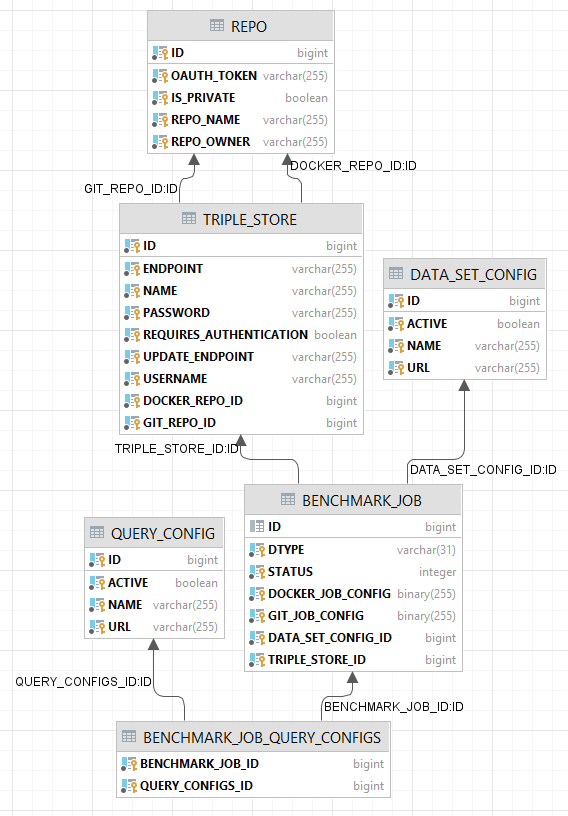
\includegraphics[width=.7\textwidth]{figures/jms_db_schema.png}
	\caption{Diagram of the previous database schema used in the \ac{jms}}
	\label{fig:jms_db_schema}
\end{figure}



\subsection{Missing Implementations}
\label{sec:review_missing_impl}
The Basilisk platform was not yet fully implemented.
After reviewing the source code, the following overview was created.

\subsubsection{\acl{hcs}}
The implementation of the \acl{hcs} was well developed.
Small additions had to be implemented.

\begin{itemize}
	\item The REST endpoints for deleting \gh{} and \dockh{} repositories had to be added.
	
	\item Previously Pull Requests for \gh{} repositories could not be observed.
\end{itemize}


\subsubsection{\acl{jms}}
The implementation of the \acl{jms} was mainly missing the REST API and some internal logic.
The following REST endpoints had to be added:

\begin{itemize}
	\item Adding / removing \ts{} configurations
	
	\item Adding / removing benchmark configurations
		\begin{itemize}
			\item Adding / removing dataset configurations
			
			\item Adding / removing query configurations
		\end{itemize}
\end{itemize}

Since the \ac{jms} also manages the running and pending benchmark jobs, the REST API and internal logic for managing these jobs had to be implemented too.

\begin{itemize}
	\item List running / pending jobs and their status
	
	\item Aborting a benchmark job
\end{itemize}



\subsubsection{\acl{tbs}}
The implementation of the \acl{tbs} previously contained only a few classes for the data models, and simple structures of service classes.
Big parts of the logic had still to be implemented.

Existing classes were mainly for storing and manipulating data models, configurations and basic message queue interactions.
These classes did not carry much functionality.

The main functionality of the \ac{tbs} had to be implemented.
This consisted of setting up the Docker containers which contain the \tsp{} for benchmarking:

\begin{itemize}
	\item Pulling Code from \gh{}
	\item Pulling images form \dockh{}
	
	\item Building Docker containers from Dockerfiles / Docker Images
	
	\item Connecting to the Docker containers
\end{itemize}

Further the usage of the \iguana{} framework had to be implemented.
The framework had to be setup to write the benchmark results to the \acl{jsts}.
\\

To have a better control of the running jobs and the benchmarking service in general, we recommended to add a small REST API to the \ac{tbs}.
This API is be similar to the one of the \ac{hcs}, that starts and stops the continuous checking.
The API for the \ac{tbs} functions like a switch, which indicates if a new benchmarking job will be started or not.
If it is set to off, the current benchmarking job will be finished, but no new job will be started.

Lastly, after performing of a benchmark, the cleanup of the Docker containers had to be implemented.

\subsection{User Management and Security}
\label{sec:review_user_management}
The Basilisk platform has no user management or any kind of access control implemented.
Currently, the REST APIs of the services allow interactions with any user.
If the platform is needed to run publicly, some user management and further security measures are needed.
That includes registering new users and user groups with different user rights.
Some users should only be able to read benchmark results, while other users should be able to create repositories and abort jobs.

Secondly, confidential information need to be kept secret.
This is for example the OAuth-Key needed for accessing private \gh{} repositories.


\subsection{Frontend}
\label{sec:review_frontend}
The frontend introduces new programming languages and frameworks.
A short review of the current source code resulted in the following findings:
\begin{itemize}
	\item Currently only a small web view is implemented
	\item Functionality to communicate with the REST APIs is missing
\end{itemize}


As explained in section \ref{sec:time_schedule}, the priority for the frontend has been lowered.
The priority of the thesis lies in finishing the main services and their functionality.





